\documentclass[twocolumn]{article}
\usepackage{authblk}
\usepackage{amsmath}
\usepackage{textcomp}
\usepackage{color}
\usepackage{blindtext}
\usepackage{listings}
\usepackage{abstract}
\lstset{language=Matlab}

\begin{document}
\title{LAB ROTATION REPORT \\ }
\date{01.04.2013}
\author[1]{\c{S}eyma BAYRAK\thanks{seyma.bayrak@st.ovgu.de}}
\affil[1]{\footnotesize  Otto von Guericke University of Magdeburg}
\maketitle
\newpage

\twocolumn[
\begin{@twocolumnfalse}
\begin{abstract}

ABSC
\\ 

\end{abstract}

\end{@twocolumnfalse}  ]
 

 \section{Introduction}


 \section{Theoretical Background}
Wilson-Cowan model introduces a solution to the derivative of a time dependent activity $u(t)$ by consideriong an external input $s(t)$ in addition to Gaussian white noise $\xi(t)$ as the following;

\begin{equation}
 \tau\dot{u}(t)=-u+\Phi(u,s)+\sigma\sqrt{\tau}\xi(t)
\end{equation}
\begin{equation*}
\rightarrow du(t)=-\frac{u}{\tau}dt+\frac{1}{\tau}\Phi(u,s)dt+\frac{\sigma}{\sqrt{\tau}}n(t)\sqrt{dt} 
\end{equation*}
where $\tau$ is the time constant, $\sigma$ is the amplitute of the Gaussian white noise, and $\Phi(u,s)$ is the \textit{generalized logistic function (GLF)} depending on the input $s(t)$.

\subsection{GLF}
In order to compute the activity $u(t)$ iteratively as Wilson-Cowan model suggests, GLF must be defined properly. The generalized logistic function (GLF) is expressed below, as suggesed by Maurizio. 

\begin{equation}
 \Phi(x)=(1+e^{-\beta x+\alpha})^{-1/\nu}
\end{equation}

Either eqaution 1 or 2 are not trivial to fit the computed or expected activity $u(t)$ ideally to the experimental result plots, since they both depend on many parameters such that $\tau$, $\sigma$, $\beta$, $\alpha$ and $\nu$. Those parameters must be chosen well reasonably. My lab rotation has actually started with the analysis of GLF function, how it looks like with different parameters. This subsection reflects the shape of GLF function under change of its parameters.

 
\subsubsection{Inflection Point}
Inflection point on a curve is basically defined as the point at which curvature changes sign, or the second derivative of the curve equals to zero. When equation 2 is reduced to the form of $\Phi''(x)=0$, the inflection point's parameters seem to be as in the following:
\begin{equation*}
 x_{inflecion}=\dfrac{\alpha-\nu}{\beta},   \;\;\;\;\;\;        y_{inflection}=(1+\nu)^{-1/\nu}
\end{equation*}

\begin{center}
 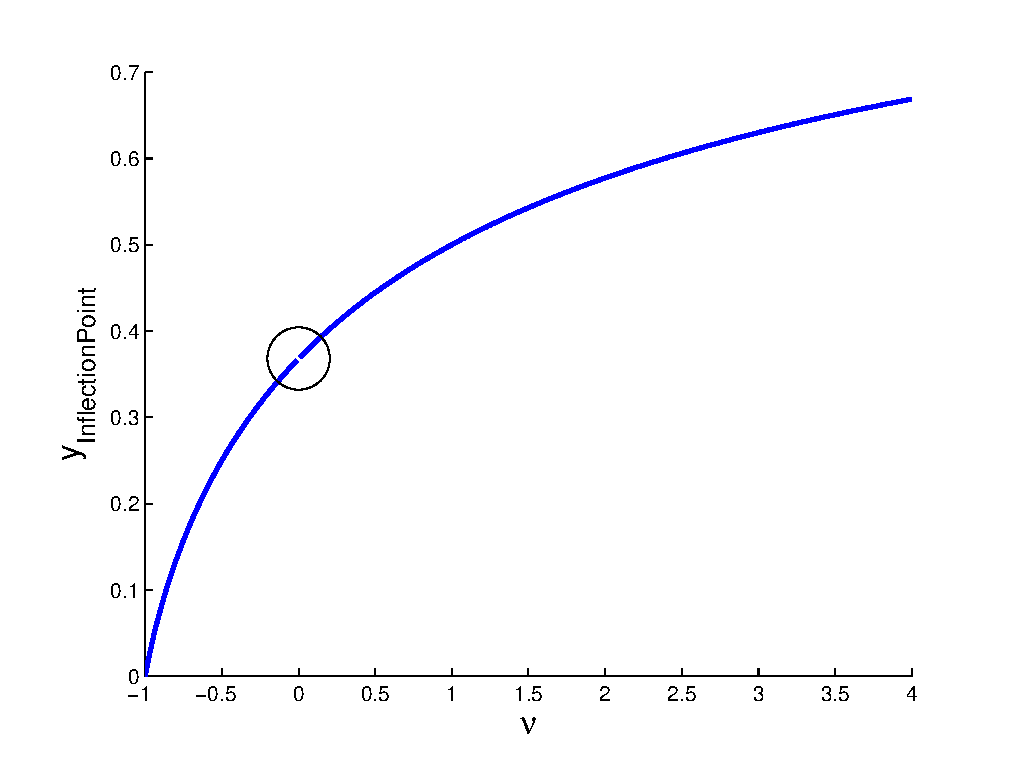
\includegraphics[width=80mm, height=60mm]{inflection_point.eps}
\begin{footnotesize}Figure 1: For each different concentration value of BSA standards, the measured absorbence values are plotted. The dashed line indcates the linear fit to the data. \end{footnotesize}
\end{center}




\end{document}
